% %!TEX root = ../main.tex
% \section{An Overview of \sys} 
% \label{sec:overview} 

% %!TEX root = ../../main.tex
\begin{figure}[t]
    \centering 
    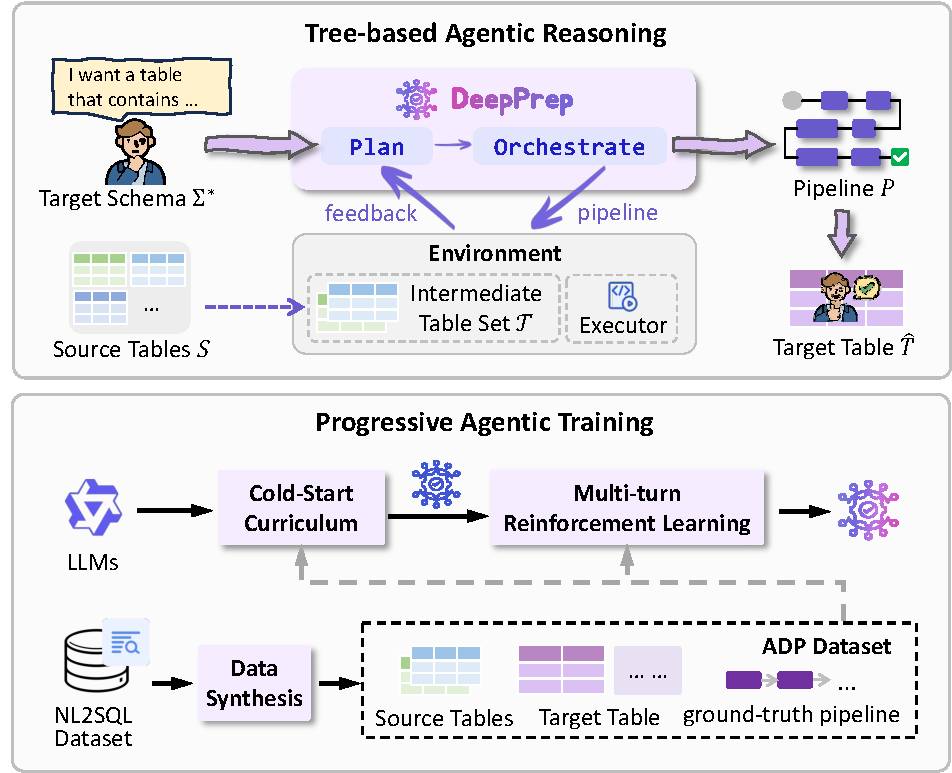
\includegraphics[width=0.9\columnwidth]{figures/fig/framework_overview.pdf}
   \vspace{-1em}
    \caption{An overview of \sys.
    }
    \label{fig:framework_overview}
   \vspace{-1em}
\end{figure}
% % %!TEX root = ../../main.tex
\begin{figure}[t]
    \centering 
    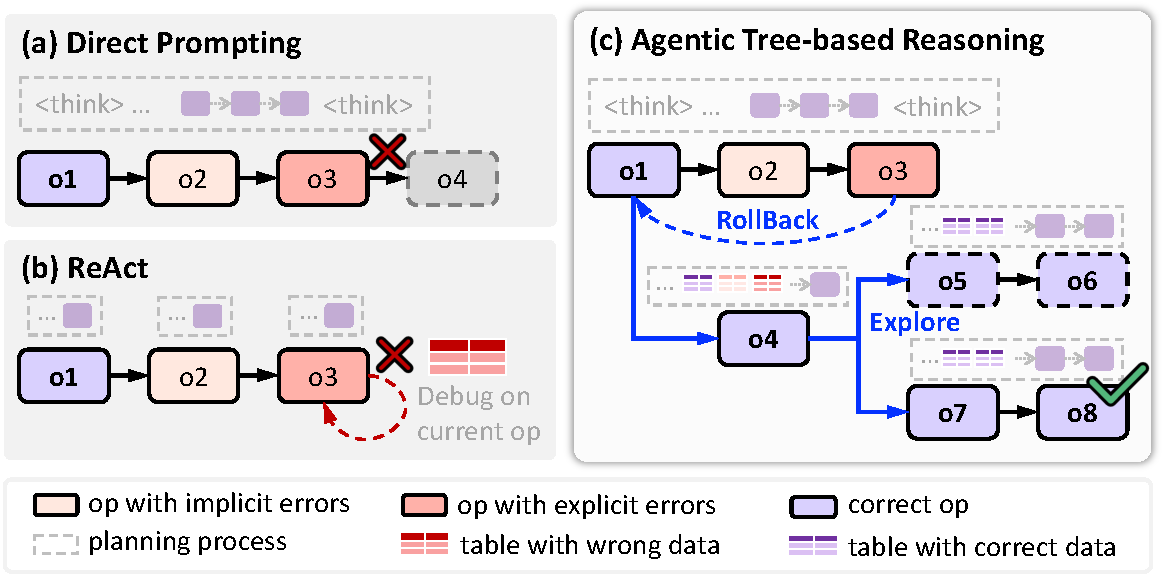
\includegraphics[width=0.99\columnwidth]{figures/fig/prompting_methods.pdf}
    % \vspace{-1em}
    \caption{Comparison of Different Inference Engine.
    }
    \label{fig:prompting_methods}
    % \vspace{-1em}
\end{figure}

% Our \sys consists of a operation orchestration framework \promptframework, a data synthesis method \datasyn and a policy learning framework \policylearn.

% \subsection{The Operation Orchestration Framework.} 

% The main goal of this paper is to propose an efficient operation orchestration to address the inherent compositional complexity challenge. To this end, we define a Tree-based Operation Orchestration framework (\promptframework) for \sys, which first generates a operation tree in multiple turns and finally extracts a sequence of operations as solution to transform input tables into the queried target table as shown in Figure~\ref{fig:framework_overview}.

% Formally, consider an table transformation task of an NL description $Q$ and input tables $D$. At the beginning, we set the operation tree $\mathcal{T}$ to empty for initialization. Then, for each turn, \promptframework analyzes the table transformation task and the current operation tree (defined as $\mathcal{T}$) to generate a new sequence of operations. The generated operations will be integrated as a new branch to update $\mathcal{T}$. Finally, \promptframework will extract a transformation pipeline $\Pi$ based the operation tree $\mathcal{T}$ to produce a generated table $\hat{T^*}$.

% % Figure~\ref{fig:prompting_methods} illustrates the basic idea of \promptframework and previous popular prompting framework. Our proposed \promptframework demonstrates two main advantages:

% This design endows our framework with two capabilities:

% \bi
% \item[(1)] \etitle{Exploration.} When the next correct transformation operation is unclear in a certain state, the model can extend multiple branches from the current node, explore various possible paths, and select the correct branch based on the execution result. For example, in Figure~\ref{fig:introduction_example}, we need to convert the \textit{ratings} table into a metric table of the ratings for specified years. The model will attempt to directly add columns by operation \texttt{AddColumn}, generate code using \texttt{ExeCode} to complete this conversion and use operation \texttt{Filter} and \texttt{Pivot} to get a pivot table. By analyzing the output of these three explorations, \promptframework selects the third one to get a correctly transformed table. 
% \item[(2)] \etitle{Rollback.} Secondly, if the correct target table can not be generated from current state due to obvious errors in the intermediate tables, the \promptframework will analyzes the operation tree $\mathcal{T}$ and then roll back to the previously erroneous node (which can be a few steps back from the current node) for debugging. Consider the example in Figure~\ref{fig:introduction_example}. In step \circled{3}, \promptframework notices that the column \texttt{genre} contains a composite movie category value ``Sci-Fi, Action''. However, directly explode current table may output repetitive records for group (``Christopher Nolan'', ``Sci-Fi'') and (``Christopher Nolan'', ``Action''). Thus, \promptframework rollback to incrementally conduct \texttt{Explode} and \texttt{Deduplicate} on previously cleaned table \textit{movies}.
% \ei

% % \stitle{Theoretical Motivation for Tree Structure.} The tree-based design is motivated by rigorous theoretical analysis of search space complexity and draws inspiration from classical AI search algorithms. Our approach fundamentally changes the search paradigm by decomposing the problem into hierarchical subproblems, following the divide-and-conquer principle~\cite{cormen2009introduction}.

% % \etitle{Divide-and-Conquer Principle.} Each subtree represents a coherent transformation module (e.g., data cleaning, table joining, aggregation), enabling independent optimization and parallel exploration. This decomposition allows the system to tackle complex transformation tasks by breaking them into smaller, manageable subproblems.

% % \etitle{Branch-and-Bound Optimization.} Our approach implements a variant of branch-and-bound search~\cite{land1960automatic}, where intermediate execution results serve as bounds for pruning unpromising branches. This is formalized through our \textit{execution-guided pruning} mechanism:

% % \begin{equation}
% % \text{Prune}(\text{branch}) = \begin{cases}
% % \text{True}, & \text{if } \text{Quality}(T_{\text{intermediate}}) < \tau \\
% % \text{False}, & \text{otherwise}
% % \end{cases}
% % \end{equation}

% % where $\text{Quality}(\cdot)$ measures intermediate table quality using our partial reward function and $\tau$ is a learned threshold.

% % \stitle{Tree-based Search Space Reduction.} Let $\mathcal{T}$ be a tree with maximum depth $d$ and branching factor $b$. The key insight is that tree-based orchestration enables \textit{early pruning} of invalid branches through intermediate execution feedback.

% % \begin{theorem}[Search Space Reduction]
% % \label{thm:search_reduction}
% % Let $p$ be the probability that a randomly chosen operation sequence of length $k$ produces a valid intermediate result. Under the tree-based orchestration with early pruning, the effective search space size is bounded by:
% % \begin{equation}
% % |\mathcal{S}_{\text{tree}}| \leq \sum_{k=1}^{d} b^k \cdot p^{k-1}
% % \end{equation}
% % \end{theorem}

% % \begin{proof}
% % At each level $k$ of the tree, we explore at most $b$ branches from each valid node. The number of valid nodes at level $k-1$ is bounded by $b^{k-1} \cdot p^{k-2}$ (since each path of length $k-1$ has probability $p^{k-2}$ of being valid). Therefore, the total number of nodes explored at level $k$ is at most $b^{k-1} \cdot p^{k-2} \cdot b = b^k \cdot p^{k-2}$. However, only a fraction $p$ of these will be valid, giving us $b^k \cdot p^{k-1}$ valid nodes at level $k$. Summing over all levels yields the bound.
% % \end{proof}

% % For typical values ($b = 3, d = 6, p = 0.3$), this reduces the search space to approximately $10^3$ nodes, representing a reduction factor of over $10^{11}$ compared to the exponential linear search space of $3.5 \times 10^{14}$ sequences (as established in Section~\ref{subsec:complexity_analysis}).

% % \stitle{Rollback Mechanism Analysis.} The rollback capability further enhances efficiency by enabling recovery from suboptimal states. Let $\mathcal{G} = (V, E)$ be the state transition graph where $V$ represents table states and $E$ represents operations. Traditional linear approaches can only move forward along paths, while our tree-based approach allows backtracking to any ancestor node.

% % \begin{definition}[Reachability Improvement]
% % The rollback mechanism increases the reachable state space from a linear path of length $l$ to a tree subgraph with up to $\sum_{i=1}^{d} b^i$ reachable states from any given starting state.
% % \end{definition}

% % This theoretical foundation demonstrates that tree-based orchestration provides both computational efficiency through search space reduction and solution quality improvement through enhanced reachability.


% \stitle{Theoretical Motivation.} The tree-based design is motivated by search space complexity analysis. Traditional linear approaches face exponential search spaces of $O(m^l)$ possible sequences, where $m$ is the number of operations and $l$ is the sequence length. Our tree-based orchestration with early pruning reduces this to approximately $O(b^d \cdot p^{d-1})$, where $b$ is branching factor, $d$ is depth, and $p$ is the probability of valid intermediate results. For typical values, this represents a reduction factor of over $10^{11}$ compared to linear approaches, while enabling rollback capabilities that increase solution reachability. A complete proof can be found in our technical report~\ref{technical_report}.

% % \stitle{Technical Design.} 

% However, to train a well-performed operation orchestration framework defined as above requires several technical designs. In this paper, we propose \datasyn and \policylearn module as technical support for \promptframework as shown in Figure~\ref{fig:framework_overview}.

% \subsection{Technical Designs}

% \stitle{(1) Data Synthesis.} We utilize realistic source tables and target tables in public NL2SQL dataset, since they reflect the real data demands. Moreover, under the table transformation settings, we require to consider more data transformation operations beyond SQL operators. Thus, our data systhesis consists of two stages: Forward Generation to convert SQL to operations defined in table~\ref{tbl:operator_space} and Backward Generation to conduct inverse operations on source tables to get non-relational table tables containing dirty data. Finally, we can generate end2end data under our table transformation setting, which can be used as supervision for afterwards policy learning. More details of the data synthesis method are given in Section~\ref{sec:data_synthesis}.

% \stitle{(2) Policy Learning.} Building on the synthesized data, we first conduct Cold Start SFT on initialized policy. Specifically, we conduct warmup training to get the policy model used to operations defined in table~\ref{tbl:operator_space} and generate multi-solution trajectory data to sft warmup policy to follow the instructions of \promptframework. Next, we construct a hybrid Reward consisting of heuristic reward, partial reward and LLM-as-Judge reward to conduct multiturn reinforcement learning on cold started policy to enhance its reasoning capabilities for performance improvement. More details of the training framework will be given in Section~\ref{sec:agentic_training_framework}.

% Together, the two modules ensure the capabilities of explore and rollback for \promptframework, enabling efficient operation orchestration for end2end table transformation task.



%!TEX root = ../main.tex
\section{An Overview of \sys} 
\label{sec:overview} 

%!TEX root = ../../main.tex
\begin{figure}[t]
    \centering 
    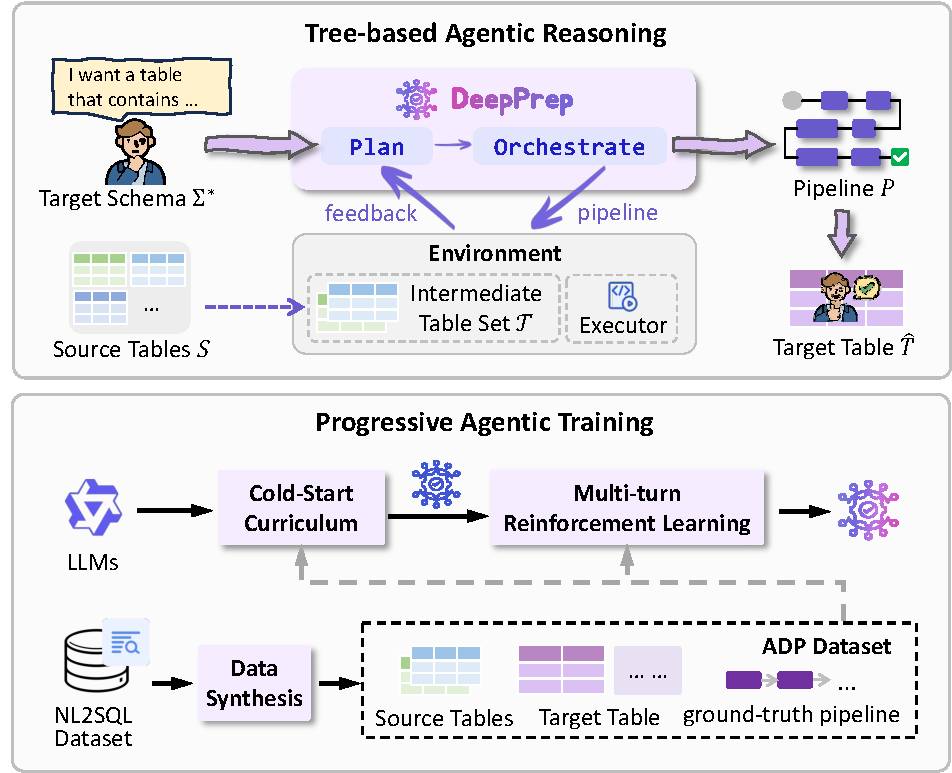
\includegraphics[width=0.9\columnwidth]{figures/fig/framework_overview.pdf}
   \vspace{-1em}
    \caption{An overview of \sys.
    }
    \label{fig:framework_overview}
   \vspace{-1em}
\end{figure}

To address the core challenge of compositional complexity in NL-\nlwhat data preparation, we propose \sys, a unified end-to-end framework. As illustrated in Figure~\ref{fig:framework_overview}, \sys is built upon three core innovations designed to work in concert:

\stitle{A Tree-based Operation Orchestration Framework (\promptframework):} This is the central reasoning engine of \sys. Instead of generating a linear sequence of operations, it constructs a transformation tree, enabling dynamic exploration of different transformation paths and intelligent backtracking from errors. This novel structure is designed to navigate the vast search space efficiently. We will detail this framework in Section~\ref{sec:framework}.
    
\stitle{Bi-Directional Full-Chain Supervision Synthesis (\datasyn):} To overcome the scarcity of training data, we introduce a data synthesis pipeline that generates high-quality, full-chain supervision examples. This component is crucial for training a model capable of handling complex, multi-step transformations. The synthesis process is described in Section~\ref{sec:data_synthesis}.
    
\stitle{Multi-Stage Policy Learning (\policylearn):} To effectively train our orchestration model, we employ a sophisticated policy learning strategy. This begins with a multi-stage cold start to bootstrap the model's capabilities and is followed by multiturn reinforcement learning with a hybrid reward function to refine its complex reasoning abilities. This learning framework is elaborated in Section~\ref{sec:agentic_training_framework}.

Together, these components empower \sys to deconstruct complex natural language requests into manageable, executable transformation plans, robustly handling the long-chain, multi-step nature of real-world data preparation tasks.